\documentclass[remotesensing,article,submit,moreauthors,pdftex]{Definitions/mdpi}

\firstpage{1}
\makeatletter
\setcounter{page}{\@firstpage}
\makeatother
\pubvolume{xx}
\issuenum{1}
\articlenumber{5}
\pubyear{2019}
\copyrightyear{2019}
\history{Received: date; Accepted: date; Published: date}

\usepackage{colortbl}
\usepackage{breakcites}
\usepackage{float}
\usepackage{graphicx}
\usepackage{amsmath}
\newcommand{\inlineeqnum}{\refstepcounter{equation}~~\mbox{(\theequation)}}
\usepackage{enumitem}
\usepackage[ruled,vlined]{algorithm2e}
\usepackage{booktabs}
\usepackage{pgfplotstable}
\pgfplotsset{compat=1.14}
\usepackage{longtable}
\usepackage{tabu}
\usepackage{hyperref}

\Title{Imbalanced Learning in Land Cover Classification:  \\ \LARGE{Improving
minority classes' prediction accuracy using the Geometric SMOTE algorithm}}
\Author{Georgios Douzas $^{1}$, Fernando Bacao$^{1}$*, Joao Fonseca
$^{1,\dagger}$ and Manvel Khudinyan $^{1,\dagger}$} \AuthorNames{Georgios
Douzas, Fernando Bacao, Joao Fonseca and Manvel Khudinyan} \address{$^{1}$ \quad
NOVA Information Management School; \{gdouzas, bacao, jpfonseca,
mkhudinyan\}@novaims.unl.pt}
\corres{Correspondence: bacao@novaims.unl.pt; Tel.: +351 21 382 8610}
\firstnote{These authors contributed equally to this work.}

\abstract{The automatic production of Land Use/Land Cover maps continues to be
a challenging problem, with important impacts on the ability to promote
sustainability and good resource management. The ability to build robust
automatic classifiers and produce accurate maps can have a significant impact
on the way we manage and optimize natural resources. The difficulty in
achieving these results comes from many different factors, such as data quality
and uncertainty. In this paper, we address the imbalanced learning problem, a
common and difficult conundrum in remote sensing that affects the quality of
classification results by proposing Geometric-SMOTE, a novel oversampling
method, as a tool for addressing the imbalanced learning problem in remote
sensing. Geometric-SMOTE is a sophisticated oversampling algorithm which
increases the quality of the generated instances over previous methods, such as
the Synthetic Minority Oversampling TEchnique. The performance of Geometric-
SMOTE, in the LUCAS (Land Use/Cover Area frame Survey) dataset, is compared to
other oversamplers using a variety of classifiers. The results show that
Geometric-SMOTE significantly outperforms all the other oversamplers and
improves the robustness of the classifiers. These results indicate that, when
using imbalanced datasets, remote sensing researchers should consider the use
of these new generation oversamplers to increase the quality of the
classification results.}

\keyword{Imbalanced learning; LULC classification; Oversampling;
Geometric-SMOTE; Class imbalance;}

\begin{document}

\section{Introduction}
The production of accurate Land Use/Land Cover (LULC) maps offers unique
monitoring capabilities within the remote sensing domain \cite{Mellor2015}. LULC
maps are being used for a variety of applications, ranging from environmental
monitoring, land change detection, natural hazard assessment up to agriculture
and water/wetland monitoring \cite{Khatami2016}, therefore, accurate and timely
production of LULC maps is of great significance. LULC maps are usually
produced by two main procedures: photo-interpretation by the human eye, which is
time and resource consuming and is not suitable for operational LULC-mapping
over large areas, and second, automatic mapping using remotely sensed data and
different classification algorithms.

The availability and a swift update of high-quality satellite remote sensing
data has brought tremendous progress in providing up-to-date and accurate land
cover information. Multispectral images, particularly, are an essential
resource to build LULC maps, allowing for the use of classification algorithms
to automate their production. Although significant progress has been made in
the use of supervised learning techniques for automatic image classification
\cite{Tewkesbury2015}, the acquisition of labeled training sets continues to be
a bottleneck \cite{Rajan2008}. In order to build accurate and robust supervised
classifiers it is crucial to have a large enough training dataset. Often, the
problem is that different land cover types have very different levels of area
coverage, which causes some of them to be frequent in the training dataset,
while others are limited \cite{Feng2019}.

A particular case where this phenomenon happens is the LUCAS dataset: Land Use
and Coverage Area frame Survey coordinated by The Statistical Office of the
European Commission (Eurostat) \cite{LUCAS2015C1}. LUCAS surveys have been
carried out every three-years since 2006 and are freely accessible  For this
statistical sampling survey a 2 km regular grid is implemented, and over
1,000,000 points were observed in the European Union territory for the year of
2015. Although, the LUCAS dataset is designed for  statistical estimation, some
existing studies are using this data for training machine learning classifiers
for land cover classification successfully \cite{Pflugmacher2019, Mack2017},
since each of the observation is empirically registered in the field (in-situ).
This sampling strategy is particularly interesting for this research, as it
causes uneven representation of different land cover classes in the dataset for
the given area.

The above-mentioned asymmetry in class distribution affects the performance of
classifiers negatively. In the machine learning community, the problem is known
as imbalanced learning problem \cite{Chawla2004}. The imbalanced learning
problem generally refers to a skewed distribution of data across classes in
both binary and multi-class problems \cite{Abdi2016}.The latter, in particular,
appears to be an even more challenging task \cite{Garcia2018}. In both cases,
during the learning phase, the minority class(es) contribute less to the
minimization of accuracy, the typical objective function, inducing a bias
towards the majority class. Consequently, as typical classification algorithms
are designed to work with reasonably balanced datasets, learning the decision
boundaries between different classes becomes a very difficult task
\cite{Saez2016}.

The possible approaches to deal with the class imbalance problem can be divided
into three main groups \cite{Fernandez2013}:

\begin{enumerate}

	\item Cost-sensitive solutions. They introduce a cost matrix that applies
	      higher misclassification costs for the examples of the minority class.

	\item Algorithmic level solutions. They modify the algorithmic procedure to
	      reinforce the learning of the minority class.

	\item Resampling solutions. They rebalance the class distribution either by
	      removing instances from the majority class or by generating artificial
				data for the minority class(es).

\end{enumerate}

The latter method constitutes a more general approach since it can be used for
any classification algorithm and it does not require any type of domain
knowledge in order to construct a cost matrix.

There are several resampling solutions to deal with the imbalanced learning
problem, which also can be divided into three categories:

\begin{enumerate}

	\item Undersampling algorithms reduce the size of the majority class.

	\item Oversampling algorithms attempt to even the distributions by
	      generating artificial data for the minority class(es).

	\item Hybrid approaches use both oversampling and undersampling techniques
	      to ensure a balanced dataset.

\end{enumerate}

In this paper, we compare the performance of various oversampling algorithms on
the publicly available EUROSTAT's Land Use/Cover Area Statistical Survey
(LUCAS) dataset \cite{LUCAS2015C3} with Landsat 8 data. The experimental
procedure includes a comparison of five oversamplers using five classifiers and
three evaluation metrics. Specifically, the oversampling algorithms are
Geometric SMOTE (G-SMOTE) \cite{Douzas2019}, the Synthetic Minority
Oversampling TEchnique (SMOTE) \cite{Chawla2002}, Borderline SMOTE (B-SMOTE)
\cite{Han2005}, thr Adaptive Synthetic Sampling Technique (ADASYN)
\cite{HaiboHe2008} and Random Oversampling (ROS), while no oversampling is
included as a baseline method. Results show that G-SMOTE outperforms every
other oversampling technique, for the selected evaluation metrics.

This paper is organized in five  sections: Section 2 analyzes the resampling
methods, section 3 describes the proposed methodology, section 4 shows the
results and discussion and section 5 presents the conclusions drawn from this
study.

\section{Resampling methods}

Data modification through resampling has been the most popular approach to deal
with the imbalanced learning problems in machine learning in general and remote
sensing in particular \cite{Feng2019}. As mentioned above, by decoupling the
imbalance problem from the classification algorithms, resampling allows the
users to apply any standard algorithm once the resampling preprocessing step is
done. This stratagem is especially convenient for users that are not machine
learning experts and want to use several classifiers. Additionally, resampling
methods can be naturally applied to multi-class imbalanced data, which is
relevant for LULC classification. In this section, we present the most relevant
applications of resampling methods for remote sensing imbalanced data
classification.

\subsection{Random resampling}

Random resampling refers to non-informed strategies that remove instances from
the majority class or replicate instances from the minority class. As such, the
selection of the data occurs randomly without exploiting any additional
information.

Some of the existing remote sensing studies implement the Random Undersampling
(RUS) method \cite{Azadbakht2016}, which randomly reduces the number of the
majority class training samples. However, this method has the disadvantage of
information loss as it discards samples from the majority class
\cite{Feng2019}. Contrary to RUS, ROS is a method that can be considered as
equivalent to Bootstrapping, as it avoids information loss. However, ROS simply
replicates randomly selected instances of the minority class, increasing the
risk of overfitting \cite{Krawczyk2016}. \cite{Maxwell2018} reports that
balancing data with ROS affects the classification performance differently for
various classifiers. In their paper, land cover classification with highly
imbalanced data is carried out with six different models. The application of
ROS slightly improved the performance of the Random Forest (RF) and Support
Vector Machine (SVM) classifiers. On the other hand, it reduced the
classification accuracy for classifiers such as Decision Tree (DT), Artificial
Neural Network (ANN), K-Nearest Neighbors (KNN) and Boosted DT.

\subsection{Informed resampling}

In the above section, the disadvantages of RUS and ROS have been pointed out.
Informed resampling methods aim to overcome these insufficiencies. More
specifically, they use the local or global information of the class distribution to
remove or generate instances. Our focus is on oversampling algorithms, since the
size of the LUCAS dataset does not favor the use of undersampling approaches.
Additionally, \cite{Feng2018} carried out a comparative analysis of
undersamplers' and oversamplers' performance for land cover classification with
the Rotation Forest ensemble classifier, showing that oversampling methods
outperform undersampling methods.

SMOTE is the most popular informed oversampling method, and it has been used to
successfully deal with the class imbalance problem in land cover classification
\cite{Cenggoro2018}. In this approach, the minority class is oversampled by
randomly selecting a minority class instance and generating synthetic examples
along the line segment joining it with one of its minority class neighbors. A
number of studies report significant improvements in LULC mapping accuracy with
the use of SMOTE oversampling. For instance, the variational semi-supervised
learning (VSSL) proposed by \cite{Cenggoro2018} aims to deal with the imbalance
problem in LULC mapping. VSSL is a semi-supervised learning framework consisting
of a deep generative model. It allows learning successfully from both labeled
and unlabeled samples while using SMOTE to balance the data. \cite{Johnson2016}
used OpenStreetMap crowdsourced data and Landsat time series for LULC
classification. Similarly, the application of SMOTE improved the classification
results. Other examples of the successful application of SMOTE in remote sensing
can be found in \cite{Bogner2018}, \cite{Panda2018}.

Although recent studies demonstrate the usefulness of SMOTE for remote sensing
applications, it still has some drawbacks. The SMOTE algorithm has the
disadvantage of generating noisy data \cite{Douzas2017}. In order to mitigate
this problem many variations of SMOTE have been developed. B-SMOTE is one of
the most popular SMOTE-based oversamplers. Similarly to SMOTE, it uses the $k$-
nearest neighbors selection strategy. The main difference to the original
algorithm is that it modifies the data generation mechanism by generating
samples closer to the decision boundary. B-SMOTE has also been reported to
perform better than SMOTE in a number of studies \cite{Nguyen2009,
Ramentol2012}. ADASYN is another well-known variation of SMOTE. It is based on
the idea of adaptively generating minority class instances according to their
weighted distribution: more instances are generated for those minority class
instances that are harder to learn compared to ones that are easier to learn
\cite{HaiboHe2008}.

The SMOTE algorithm can be decomposed into two parts: the selection strategy
for the minority class instances and the data generation mechanism. The first
part is related to the generation of noisy instances since the SMOTE selection
strategy considers all the minority samples as equivalent. The above-mentioned
SMOTE variations (B-SMOTE and ADASYN) aim to deal with this problem. On the
other hand, the second part is responsible for the diversity of the artificial
instances. There are scenarios where the linear interpolation mechanism used in
SMOTE generates nearly duplicate instances that may lead to overfitting. The G-
SMOTE algorithm is an extension of SMOTE that aims to deal with both problems.
G-SMOTE defines a flexible geometric region around each minority class instance
for synthetic data generation. The shape of this area is controlled by a set of
hyperparameters. This element significantly increases the diversity of
generated instances. Furthermore, G-SMOTE is designed to avoid noisy sample
generation since it modifies the SMOTE selection strategy. G-SMOTE has been
shown to outperform SMOTE and its above  mentioned variations across 69
imbalanced datasets for various classifiers and evaluation metrics. Figure
\ref{fig:gsmote_smote} depicts the data generation mechanism of both SMOTE and
G-SMOTE using a deformed geometric region.

\begin{figure}[H]
	\centering
	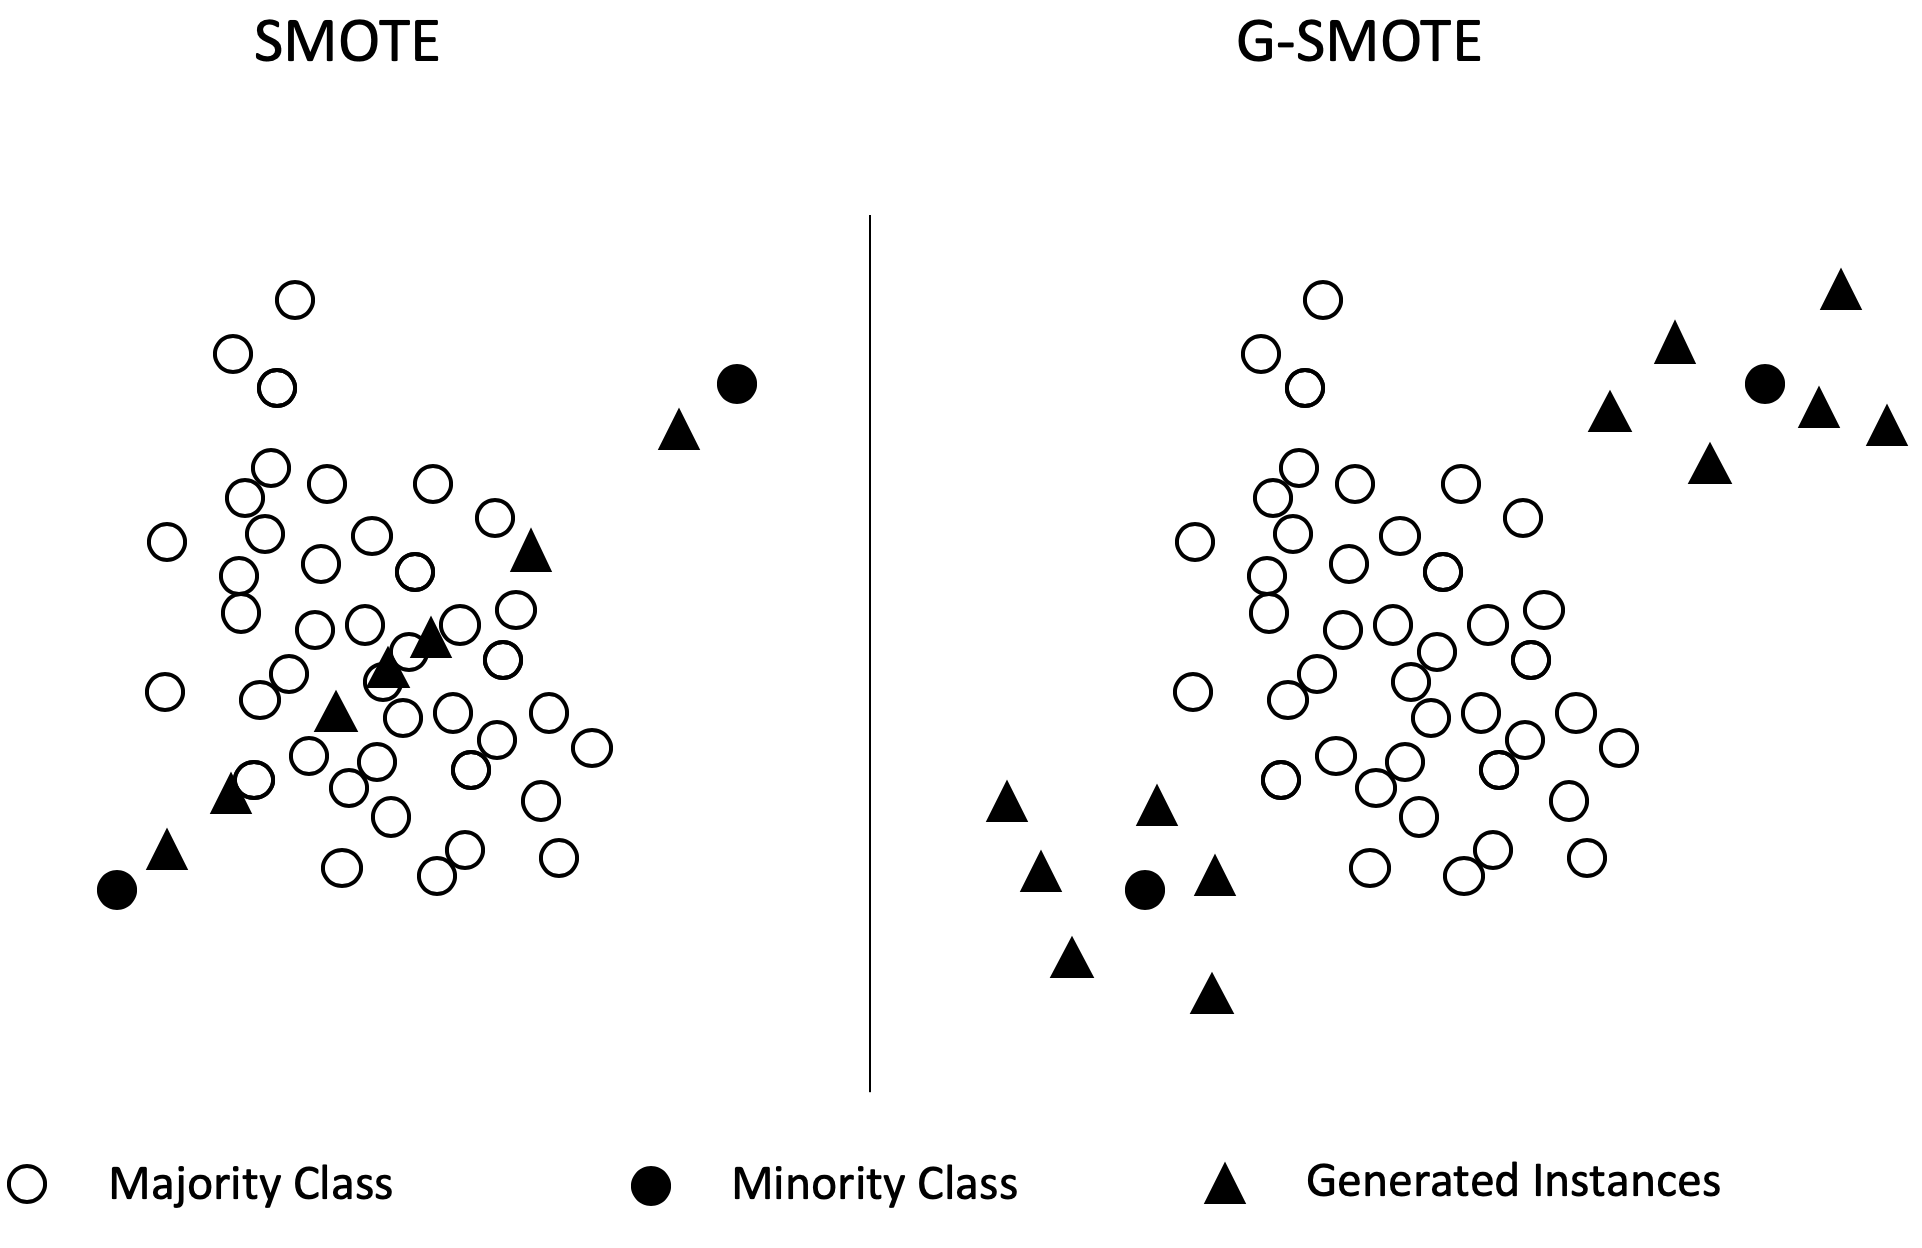
\includegraphics[width=1\linewidth]{../analysis/gsmote_smote}
	\caption{Example of minority class oversampled by SMOTE and G-SMOTE
		algorithms. G-SMOTE generates non-noisy samples
		with greater variety than SMOTE.}
	\label{fig:gsmote_smote}
\end{figure}

\section{Methodology}

This section describes the evaluation process of G-SMOTE's performance. A
description of the study area, dataset, oversamplers, classifiers, evaluation
metrics as well as the experimental procedure is provided. Figure
\ref{fig:flowchart} represents the flowchart of the steps applied in this
experiment.

\begin{figure}[H]
	\centering
	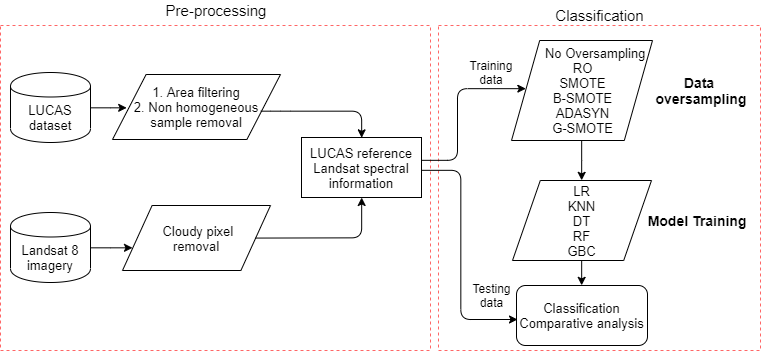
\includegraphics[width=1\linewidth]{../analysis/g_smote_flow_chart}
	\caption{Flowchart containing the steps applied in the entire method.}
	\label{fig:flowchart}
\end{figure}

\subsection{Study area}

The area of study is in north-western Portugal, corresponding to the area
covered by the Landsat 8 image from track 204 and row 32, shown in figure
\ref{fig:studyarea}. The area contains all eight  main land cover types defined
by LUCAS 2015: artificial land, cropland, woodland, shrubland, grassland, bare
land, water and wetlands.

\begin{figure}[H]
	\centering
	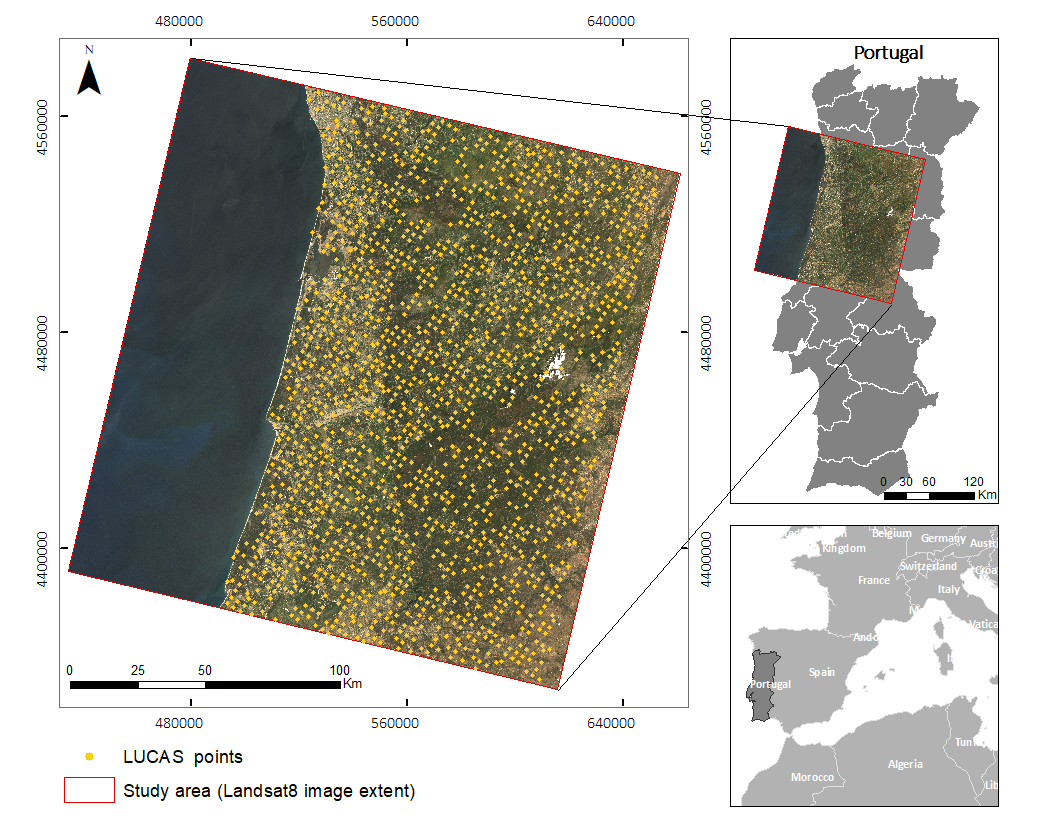
\includegraphics[width=1\linewidth]{../analysis/study_area}
	\caption{Study area and LUCAS reference data (coordinate system:
		WGS-84 UTM Zone 29, projection: Transverse-Mercator, Landsat image
		acquisition date: 2015/05/25).}
	\label{fig:studyarea}
\end{figure}

\subsection{Remote sensing data}

The remotely sensed data includes eight images from the moderate-resolution
Landsat  8 multi-spectral sensor. The images are Level-2 surface reflectance
product (OLI/TIRS); One image was acquired each month from February to
September 2015. The acquisition mode is Descending. Data were pre-processed
in order to remove pixels with cloud cover. Only bands 2, 3, 4, 5, 6, and 7
are used from each image. Accordingly, each reference point from the LUCAS
dataset has 48 features, representing pixel values from each spectral band
from each image.

\subsection{LUCAS dataset}

The 2015 LUCAS data was used as reference data for both model training and
validation. The LUCAS point label represents the corresponding land cover/use
type within the radius of 1.5 m for homogeneous classes and a 20 m radius
extent ("extended window") for heterogeneous classes (e.g., shrubland), gathered
by field observation and a very high-resolution photo interpretation
\cite{LUCAS2015C1}. In order to reduce the risk of having Landsat pixel
information represented wrongly in the field, we only kept points observed
in-situ from a close distance (<100 m). With the same objective we removed the
points which had linear features in the observation (e.g., roads).
This procedure was not solely applied to the class of "artificial land," as
this would remove most parts of the samples. Furthermore, points with cloudy
pixels in the Landsat data were also excluded. This way, 1694 out of 2060
LUCAS points were retained. This dataset contains eight classes that
represent the main land cover types for the study area

This pixel selection excluded a large number of unacceptable reference points,
and we assumed the remaining ones to be suitable enough to represent the land
cover type in a Landsat pixel coverage area of 30x30 m. Further, we surmised
that classifiers are capable of overcoming the noise caused by pixels having
mixed land cover representation if such pixels are still available in the
dataset.

The number of samples per class and the Imbalance Ratio (IR), defined as the
ratio of the number of samples for the majority class over the number of samples for
any of the minority classes, is presented in Table
\ref{tab:classes_distribution}.

\begin{table}[H]
	\centering
	\begin{tabular}{llrrrr}
		\toprule
		\textbf{LUCAS Category} & \textbf{Land cover type} & \textbf{Instances}
		                        & \textbf{IR}                                   \\
		\hline
		A                       & Artificial land          & 131
		                        & 5.81                                          \\
		B                       & Cropland                 & 270
		                        & 2.81                                          \\
		C                       & Woodland                 & 761
		                        & 1.00                                          \\
		D                       & Shrubland                & 296
		                        & 2.61                                          \\
		E                       & Grassland                & 185
		                        & 4.11                                          \\
		F                       & Bareland                 & 37
		                        & 20.56                                         \\
		G                       & Water                    & 10
		                        & 76.10                                         \\
		H                       & Wetlands                 & 4
		                        & 190.25                                        \\
		\bottomrule
	\end{tabular}
	\caption{\label{tab:classes_distribution}LUCAS nomenclature and classes
		distribution.}
\end{table}

Table \ref{tab:LUCAS} presents a description of the LUCAS dataset, including
information about the majority class C and the smallest minority class H to
emphasize the imbalance character of the dataset:

\pgfplotstabletypeset[
	begin table=\begin{longtable},
		end table=\end{longtable},
	col sep=comma,
	header=true,
	columns={Dataset, LUCAS},
	columns/Dataset/.style={column type=l,string type},
	columns/LUCAS/.style={column type=l,string type},
	every head row/.style={before row=\toprule, after row=\midrule\endhead},
	every last row/.style={after row=\bottomrule
			\caption{\label{tab:LUCAS}Description of the LUCAS dataset.}}
]
{../analysis/dataset_descrip.csv}

\subsection{Evaluation metrics}  \label{Evaluation metrics}

Amongst the possible choices existing for classifier's performance evaluation,
\textit{Accuracy}, user's accuracy (or \textit{Precision}) and
producer's accuracy (or \textit{Recall}) are the most common in LULC
classification \cite{Liu2007, Olofsson2013}. For a binary classification task,
their calculation is given in terms of the true positives \( TP \), true
negatives \(TN \), false positives \( FP \), and false negatives \( FN \)
\cite{Liu2007}. More specifically,  \( \textit{Precision} =  \frac{TP}{TP + FP}
\) and \(\textit{Recall} =  \frac{TP}{TP + FN} \). For the multi-class case, the
average value across classes is used, as explained below.

The LUCAS dataset is highly imbalanced, having a wide range of IRs for the
different minority classes. Therefore, the use of the metrics above is not an
appropriate choice since they are mainly determined by the majority class
contribution \cite{He2009}. An appropriate evaluation metric should consider the
classification accuracy of all classes. A simple approach for the multi-class
case is to select a binary class evaluation metric, apply it to each binary
sub-task of the multi-class problem, i.e., consider each class versus the rest
and finally average its values. For this purpose, \textit{F-score} and
\textit{G-mean} metrics are used as the primary evaluation methods while
\textit{Accuracy} is provided for discussion:

\begin{itemize}

	\renewcommand\labelitemi{--}

	\item The \textit{Accuracy} is the number of correctly classified
	      samples divided by the sum of all samples. Assuming that the various classes
	      are labeled by the index \( c \), \textit{Accuracy} is given by the
	      following formula:

	      $$\textit{Accuracy} = \frac{ \sum\limits_{c}{ \text{TP}_{c} } }{
			      \sum\limits_{c}{ (\text{TP}_{c}  + \text{FP}_{c}) } } $$

	\item The \textit{F-score} is the harmonic mean of \textit{Precision} and
	      \textit{Recall}. The \textit{F-score} for the multi-class case can be
	      calculated using their average per class values \cite{He2009}:

	      $$\textit{F-score}=2\frac{\overline{Precision} \times \overline{Recall}}{\overline{Precision} +
			      \overline{Recall}}$$

	\item The \textit{G-mean} is the geometric mean of \textit{Sensitivity} and
	      \textit{Specificity}. \textit{Sensitivity} is identical to the
	      \textit{Recall} while \textit{Specificity} is given by the formula
	      \(\textit{Specificity} =  \frac{TN}{TN + FP} \). Therefore, they are equal
	      to the true positive and true negative rates, respectively. The
	      \textit{G-mean} for the multi-class case can be calculated using their
	      average per class values:

	      $$\textit{G-mean} = \sqrt{ \overline{Sensitivity} \times
			      \overline{Specificity}}$$

\end{itemize}

\subsection{Machine learning algorithms}

The main objective of the paper is to show the effectiveness of G-SMOTE when it
is used on multi-class highly imbalanced data of a remote sensing application as
well as to compare its performance to other oversampling methods. Four
oversampling algorithms were used in the experiment along with G-SMOTE. ROS was
chosen for its simplicity. SMOTE was selected for being the most widely used
oversampler. ADASYN and B-SMOTE were selected for representing popular
modifications of the original SMOTE algorithm. Finally, no oversampling was also
applied as an additional baseline method.

For the evaluation of the oversampling methods, the classifiers Logistic
Regression (LR) \cite{McCullagh1989}, K-Nearest Neighbors (KNN)
\cite{Cover1967}, Decision Tree (DT) \cite{Salzberg1994}, Gradient Boosting
Classifier (GBC) \cite{Friedman2001} and Random Forest (RF) \cite{Liaw2002} were
selected. The choice of classifiers was made according to the following
criteria: learning type, training time, and popularity within the remote sensing
community. All these algorithms were found to be computationally efficient and
commonly used for the proposed task, with the exception of LR, which is rarely
used in remote sensing applications \cite{Khatami2016, Maxwell2018}.

\subsection{Experiment settings}

In order to evaluate the performance of each oversampler, every possible
combination of oversampler, classifier, and metric is formed. The evaluation
score for each of the above combinations is generated through an \( n \)-fold
cross-validation procedure with \( n = 3 \). Before starting the training of
each classifier, and in each stage \(i \in \{1, 2 ,... , n \} \) of the \( n
\)-fold cross-validation procedure, synthetic data \( S_{i} \) were generated
using the oversampler, based on the training data \(T_{i} \) of the \( n - 1 \)
folds, such that the resulting \(S_{i} \cup T_{i} \) training set becomes
perfectly balanced. This enhanced training set, in turn, was used to train the
classifier. The performance evaluation of the classifiers was done on the
validation data \( V_{i} \) of the remaining fold, where \(V_{i} \cup T_{i} = D
\), \(V_{i} \cap T_{i} = \emptyset \) while \( D \) represents the dataset. The
process above is repeated three times and the results are averaged.

The range of hyperparameters used for each classifier and oversampler are
presented in table \ref{tab:grid}:

\begin{table}[H]
	\centering
	\begin{tabular}{lll}
		\toprule
		Classifier       & Hyperparameters      & Values                       \\
		\hline
		LR               & maximum iterations   & 10000                        \\
		KNN              & number of neighbors  & {3, 5}                       \\
		DT               & maximum depth        & {3, 6}                       \\
		GBC              & maximum depth        & {3, 6}                       \\
		                 & number of estimators & {50, 100}                    \\
		RF               & maximum depth        & {None, 3, 6}                 \\
		                 & number of estimators & {50, 100}                    \\
		\toprule
		Oversampler      &                      &                              \\
		\hline
		G-SMOTE          & number of neighbors  & {3, 5}                       \\
		                 & selection strategy   & combined, minority, majority \\
		                 & truncation factor    & {-1.0, -0.5, .0, 0.25, 0.5,
				0.75, 1.0}                                                             \\
		                 & deformation factor   & {0, 0.2, 0.4, 0.5, 0.6, 0.8,
				1.0}                                                                   \\
		SMOTE            & number of neighbors  & {3, 5}                       \\
		BORDERLINE SMOTE & number of neighbors  & {3, 5}                       \\
		ADASYN           & number of neighbors  & {2, 3}                       \\
		\bottomrule
	\end{tabular}
	\caption{\label{tab:grid}Hyperpameters grid.}
\end{table}

\subsection{Software implementation}

The implementation of the experimental procedure was based on the Python
programming language, using the
\href{https://scikit-learn.org/stable/}{Scikit-Learn} \cite{Pedregosa2011},
\href{https://imbalanced-learn.org/en/stable/}{Imbalanced-Learn} \cite{JMLR:v18:16-365},
and
\href{https://geometric-smote.readthedocs.io/en/latest/?badge=latest}{Geometric-SMOTE}
libraries. All functions, algorithms, experiments and results reported are
provided at the GitHub repository of the
\href{https://github.com/AlgoWit/publications/tree/master/remote-sensing-lucas}{project}.
Additionally, the
\href{https://research-learn.readthedocs.io/en/latest/?badge=latest}{Research-Learn}
library provides a framework to implement comparative experiments, also being
fully integrated with the Scikit-Learn ecosystem.

\section{Results and discussion}

This section presents the results and analyses of oversamplers comparisons on the
LUCAS dataset. The classification results are shown for all
combinations of oversamplers and classifiers used in the experiment. The next subsection
covers their interpretation in detail.

\subsection{Results}

For each combination of classifier and metric, a cross-validation score for all
oversamplers is provided in Table \ref{tab:mean_cross_val}:

\pgfplotstabletypeset[
	begin table=\begin{longtable},
		end table=\end{longtable},
	col sep=comma,
	header=true,
	columns={Classifier,Metric,NONE,ROS,SMOTE,B-SMOTE,ADASYN,G-SMOTE},
	columns/Classifier/.style={column type=l,string type},
	columns/Metric/.style={column type=l,string type},
	columns/NONE/.style={column type=l,string type},
	columns/ROS/.style={column type=l,string type},
	columns/SMOTE/.style={column type=l,string type},
	columns/B-SMOTE/.style={column type=l,string type},
	columns/ADASYN/.style={column type=l,string type},
	columns/G-SMOTE/.style={column type=l,string type},
	every head row/.style={before row=\toprule, after row=\midrule\endhead},
	every last row/.style={after row=\bottomrule
			\caption{\label{tab:mean_cross_val}Results for cross-validation scores of
				oversamplers.}}
]
{../analysis/mean_scores.csv}

A ranking score was assigned to each oversampling method with the best and
worst- performing methods receiving scores from 1 to 6, respectively. Table
\ref{tab:mean_rankings} was created by averaging the ranking scores over all
classifiers per evaluation metric:

\pgfplotstabletypeset[
	begin table=\begin{longtable},
		end table=\end{longtable},
	col sep=comma,
	header=true,
	columns={Metric,NONE,ROS,SMOTE,B-SMOTE,ADASYN,G-SMOTE},
	columns/Metric/.style={column type=l,string type},
	columns/NONE/.style={column type=l,string type},
	columns/ROS/.style={column type=l,string type},
	columns/SMOTE/.style={column type=l,string type},
	columns/B-SMOTE/.style={column type=l,string type},
	columns/ADASYN/.style={column type=l,string type},
	columns/G-SMOTE/.style={column type=l,string type},
	every head row/.style={before row=\toprule, after row=\midrule\endhead},
	every last row/.style={after row=\bottomrule
			\caption{\label{tab:mean_rankings}Results for mean ranking of oversamplers}}
]
{../analysis/model_mean_ranking.csv}

Table \ref{tab:smote_gsmote} presents the percentage difference between G-SMOTE
and no oversampling (NONE), Random Oversampling (ROS) and SMOTE:

\pgfplotstabletypeset[
	begin table=\begin{longtable},
		end table=\end{longtable},
	col sep=comma,
	header=true,
	columns={Classifier,Metric,NONE,ROS,SMOTE},
	columns/Classifier/.style={column type=l,string type},
	columns/Metric/.style={column type=l,string type},
	columns/NONE/.style={column type=l,string type},
	columns/ROS/.style={column type=l,string type},
	columns/SMOTE/.style={column type=l,string type},
	every head row/.style={before row=\toprule, after row=\midrule\endhead},
	every last row/.style={after row=\bottomrule
			\caption{\label{tab:smote_gsmote}Results for the percentage difference
				between G-SMOTE and no oversampling (NONE), Random Oversampling (ROS)
				and SMOTE.}}
]
{../analysis/mean_perc_diff_scores.csv}

\subsection{Discussion}

From table \ref{tab:mean_cross_val}, we can observe that G-SMOTE outperforms all
other oversampling methods for both \textit{F-score} and \textit{G-mean} metrics
on all classifiers. The absolute best results are achieved when G-SMOTE is
combined with LR and RF. It is vital to notice that the \textit{Accuracy} scores
show the well-known bias towards the majority class as discussed in
\ref{Evaluation metrics}. In a multi-class classification problem with an
imbalanced dataset, where the prediction of all the classes are of equal
importance as in many remote sensing applications, \textit{Accuracy} should be
of secondary importance compared to more robust metrics, such as \textit{F-
score} and \textit{G-mean}. Nevertheless, even for the \textit{Accuracy} metric,
G-SMOTE shows the best performance amongst the oversamplers.

In table \ref{tab:mean_rankings}, the rankings of the oversamplers are presented
and show the superiority of G-SMOTE. Although SMOTE is the most popular
oversampling method in remote sensing applications, it is clear from the tables
that it produces suboptimal results. Therefore, we decided to add a table
directly comparing the performance of G-SMOTE with NONE, ROS and SMOTE (Table
\ref{tab:smote_gsmote}), which shows that G-SMOTE systematically outperforms
the remaining oversamplers, regardless of the classifier or metric used.

This study is the first to present a systematic comparison of oversampling
algorithms in remote sensing. However, several previous studies reported results
consistent with our findings. \cite{Bogner2018} reported an increase in
\textit{F-score} and \textit{G-mean} when oversampling was applied, while
classification overall accuracy did not improve. Similarly, results obtained in
\cite{Feng2019} demonstrate increased classification performance when using
SMOTE. According to our experiment, performance can be further increased by
using G-SMOTE. A number of other studies \cite{Cenggoro2018, Maxwell2018} do not
use imbalance specific metrics, therefore it cannot be directly compared to our
results.

\section{Conclusions}

In this paper we applied G-SMOTE, a novel oversampling algorithm, on a LULC
classification problem, using a highly imbalanced multi-class dataset (LUCAS).
G-SMOTE's performance was evaluated and compared with other oversampling
methods. More specifically, ROS, SMOTE, B-SMOTE and ADASYN were the selected
oversamplers while LR, KNN, DT, GBC and RF were used as classifiers.

The experimental results show that using a G-SMOTE oversampler can significantly
improve the classification performance, resulting in higher values of \textit{F-
score} and \textit{G-mean}. Therefore, readers should consider using G-SMOTE
when accurately predicting the minority classes is of equal or higher importance
compared to the accurate prediction of the majority class. Examples of the above
case are the land cover change detections and rare land cover type
classification.

G-SMOTE can be a useful tool for remote sensing researchers and practitioners,
as it systematically outperforms the previous widely used oversamplers.
G-SMOTE is easily accessible to the users through an
\href{https://geometric-smote.readthedocs.io/en/latest/?badge=latest}{open
	source implementation}.

\vspace{6pt}

\authorcontributions{Conceptualization, F.B.; Methodology, G.D.; Software,
	G.D.; Validation, F.B., G.D.; Formal Analysis, J.F and M.K.; Writing -
	Original Draft Preparation, M.K., J.F.; Writing - Review \& Editing, F.B.,
	G.D., J.F., M.K.; Supervision, F.B.; Funding Acquisition, F.B.}

\funding{This research was funded by "Fundação para a Ciência e Tecnologia"
	(Portugal), grants' number PCIF/SSI/0102/2017 and DSAIPA/AI/0100/2018 -
	IPSTERS.}

\acknowledgments{The authors would like to thank Direção Geral do Território
	(DGT) for supporting the data used in this study.}

\conflictsofinterest{The authors declare no conflict of interest. The funders
	had no role in the design of the study; in the collection, analyses, or
	interpretation of data; in the writing of the manuscript, or in the decision to
	publish the results.}

\abbreviations{The following abbreviations are used in this manuscript:\\
	\noindent
	\begin{tabular}{@{}ll}
		OS      & Oversampling                                         \\
		CV      & Cross-Validation                                     \\
		LULC    & Land Use/Land Cover                                  \\
		LUCAS   & Land Use/Cover Area Statistical Survey               \\
		SMOTE   & Synthetic Minority Over-sampling Technique           \\
		ADASYN  & Adaptive Synthetic Sampling Technique                \\
		G-SMOTE & Geometric Synthetic Minority Over-sampling Technique \\
		B-SMOTE & Borderline Synthetic Minority Over-sampling Technique\\
		ROS     & Random Oversampling                                  \\
		NONE    & No Oversampling                                      \\
		LR      & Logistic Regression                                  \\
		KNN     & K-Nearest Neighbors                                  \\
		DT      & Decision Trees                                       \\
		GBC     & Gradient Boosting Classifier                         \\
		RF      & Random Forest                                        \\
	\end{tabular}}


\reftitle{References}

\externalbibliography{yes}
\bibliography{references}

\end{document}
